\documentclass{article}

\usepackage{arxiv}

\usepackage[utf8]{inputenc}
\usepackage[T1]{fontenc}
\usepackage{hyperref}
\usepackage{url}
\usepackage{booktabs}
\usepackage{amsfonts}
\usepackage{microtype}
\usepackage{graphicx}
\usepackage{amsmath}
\usepackage{float}
\usepackage{natbib}
\usepackage{cleveref}
\usepackage{xcolor}
\usepackage{soul}

\graphicspath{{./images/}}

\sethlcolor{yellow}
\newcommand{\red}[1]{{\color{red}#1}}
\newcommand{\todo}[1]{{\color{red}#1}}
\newcommand{\TODO}[1]{\textbf{\color{red}[TODO: #1]}}

\title{Look Where It Matters: Distilling Vision Through Explanations}

\author{
  Mattia Curri \\
  Department of Computer Science \\
  University of Bari Aldo Moro \\
  Bari, Italy \\
  \texttt{m.curri8@studenti.uniba.it} \\
}

\begin{document}
\maketitle

\begin{abstract}
Can explanations serve as a useful supervision signal for knowledge distillation in vision-language models?
We investigate this question in a plug-in replacement setting: a ViT student is trained to replace the visual module of a VLM, while the original language model remains fixed.
This setting is stricter than standalone embedding evaluation because the distilled representation must still support image-conditioned generation after it is inserted back into the multimodal pipeline.
We compare global feature reconstruction with explanation-guided token reconstruction, where Grad-CAM saliency from a frozen teacher probe weights the visual tokens that the student should match most strongly.
On Mini-ImageNet image-description prompts, three independent VLM judges compare anonymized teacher and student answers while observing the original image.
On the shared subset of 437 images for which every judge returned a valid preference for every variant, the teacher remains preferred overall; however, every explanation-guided objective improves over plain global reconstruction.
Per-judge trends and qualitative examples indicate that this gain is associated with preserving localized visual evidence and avoiding severe grounding failures, while errors requiring broader scene context remain.
These findings show that explanations provide a useful distillation signal, although the distilled visual module is not yet a faithful replacement for the teacher. The code is available at \url{https://github.com/mattiacurri/ExplanationGuidedDistillation}.
\end{abstract}


\section{Introduction}
\label{sec:intro}

Knowledge distillation usually treats the teacher signal as a target to be matched uniformly: logits, features, or token embeddings are reconstructed with little regard for which parts of the representation support the teacher's decision.
For visual models, however, explanation methods provide an additional signal: they estimate which image regions or visual tokens were most influential for a prediction.
This raises the central research question of this work: \emph{can explainability provide a useful training signal for knowledge distillation, beyond ordinary feature reconstruction?}
We study this question in a demanding setting where the distilled visual encoder is not evaluated only by representation similarity, but is plugged back into a VLM and judged through the answers that the full system generates.
The plug-in VLM evaluation is therefore a stress test for the explanation-guided distillation signal: it asks whether saliency-weighted supervision preserves information that still matters after visual features are consumed by a language model.

We study this question with Qwen2.5-VL~\citep{qwen2025vl}.
The teacher VLM provides visual-token targets, and a ViT student~\citep{dosovitskiy2021image} is trained to replace the teacher's visual module while the language model is kept fixed.
The student is smaller than the original visual pathway, but compression is not the main scientific claim.
The main claim is about supervision: explanations may identify which parts of the teacher representation are most important to preserve for downstream generation.

The proposed supervision uses a teacher-side probe to produce Grad-CAM saliency over visual tokens~\citep{selvaraju2017gradcam}.
Instead of treating all token errors equally, the explanation-guided objective weights token reconstruction by saliency.
This converts an explanation into a training signal: the student is asked to prioritize teacher features that the probe identifies as decision-relevant.
The study compares this signal against plain global MSE and against combined global-plus-explanation objectives.

\begin{figure}[t]
  \centering
  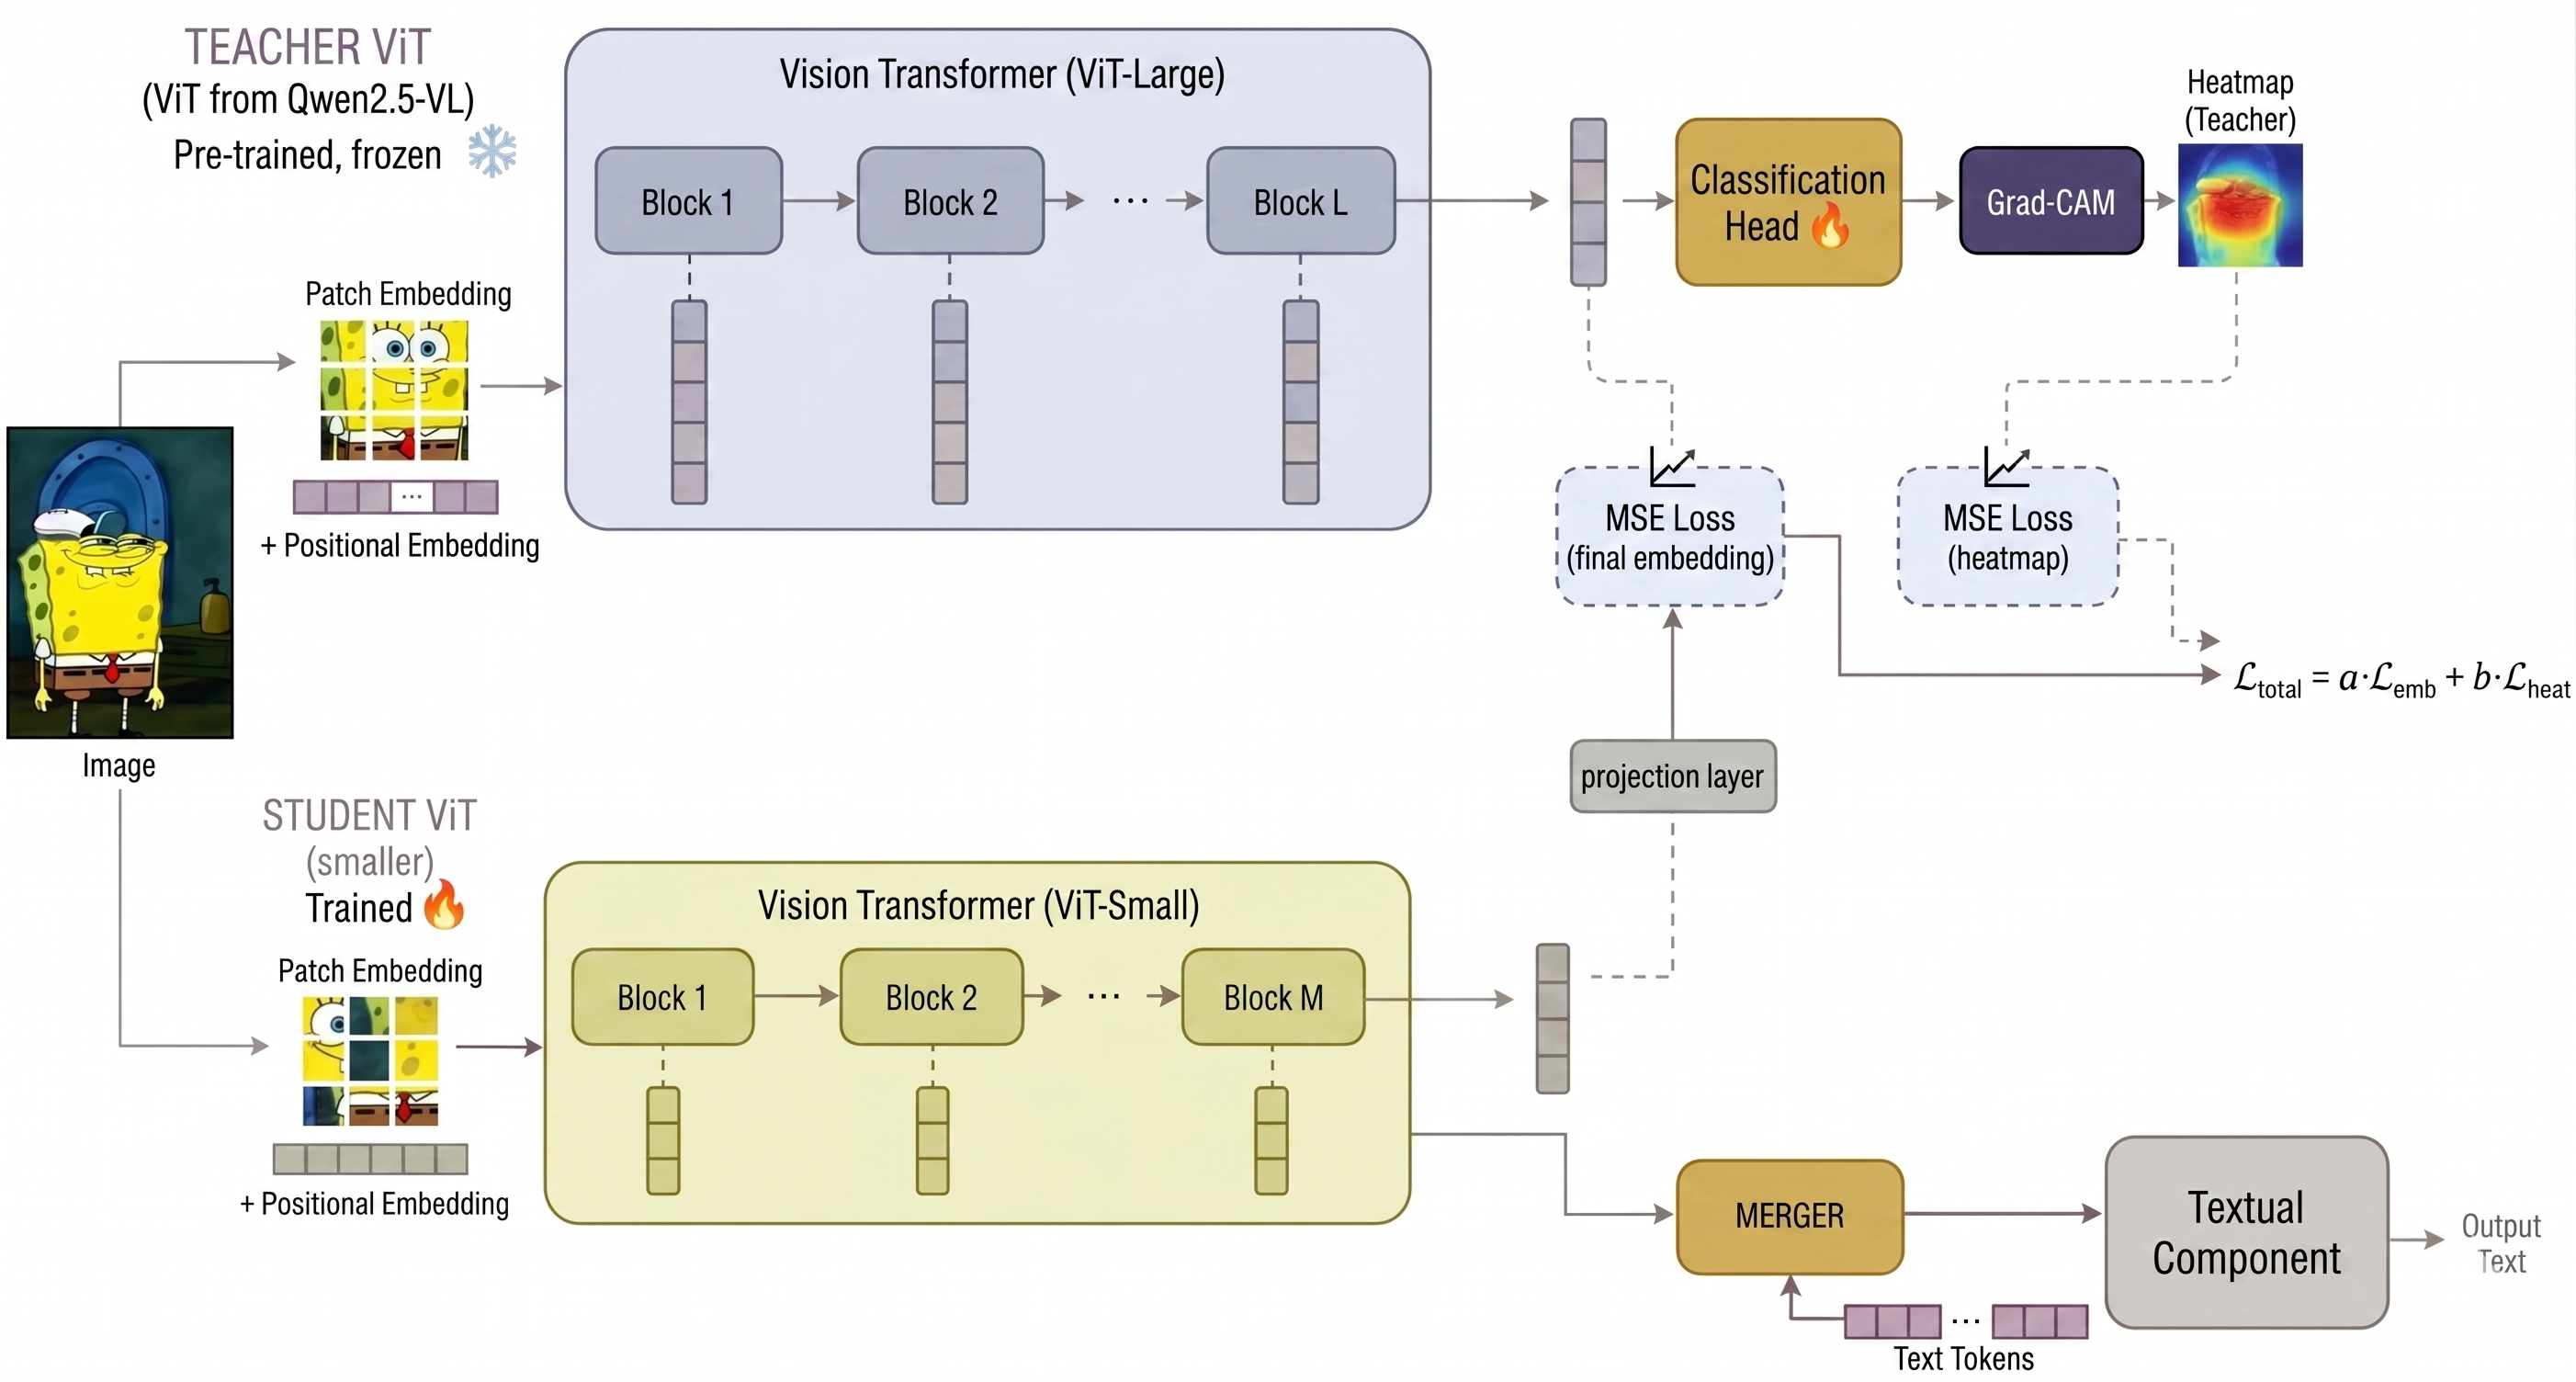
\includegraphics[width=\textwidth]{images/pipeline.png}
  \caption{Pipeline overview.}
  \label{fig:pipeline}
\end{figure}

After distillation, each student visual encoder is inserted into the same VLM generation pipeline, and the resulting answers are compared with answers from the original teacher system.
Three independent VLM judges perform blind A/B comparisons while seeing the image, so the primary metric reflects image-grounded answer preference rather than embedding similarity or text overlap alone.

The original VLM is still preferred on most examples, but the ablation shows a consistent effect of the explanation signal.
Global MSE alone produces very few student-preferred answers, whereas saliency-weighted distillation consistently improves the student preference rate.
This pattern suggests that the saliency map is not merely a visualization artifact: used as a token-level weighting signal, it changes which teacher features the student preserves, and that change remains visible in downstream VLM behavior.

The remainder of the paper is organized as follows.
Section~\ref{sec:related} situates the work relative to VLMs, visual distillation, explanation-based supervision, and generated-answer evaluation.
Section~\ref{sec:method} describes the experimental setting, teacher-probe construction, explanation-guided distillation objective, and blind image-grounded judge protocol.
Section~\ref{sec:results} reports probe quality, downstream VLM preference results, judge tendencies, and qualitative answer patterns.
Sections~\ref{sec:limitations} and~\ref{sec:conclusion} summarize the main limitations and conclusions.

\section{Related Work}
\label{sec:related}

\paragraph{Vision-language models.}
Qwen2.5-VL is an open VLM family designed for visual perception, grounding, document understanding, and instruction following~\citep{qwen2025vl}.
This work treats the VLM as the downstream system in which a distilled visual module must operate. Keeping the language model, and the merger module, fixed isolates the question of whether visual-module distillation preserves useful image evidence.
Large VLMs build on a line of work that aligns visual encoders with language supervision and then connects visual representations to text decoders or instruction-following language models.
CLIP showed that natural-language supervision can train transferable visual representations at scale~\citep{radford2021clip}.
Later architectures such as BLIP-2 and LLaVA made the interface between a visual encoder and a frozen or instruction-tuned language model a central design object~\citep{li2023blip2,liu2023llava}.
Our setting evaluates the student inside the VLM rather than treating the visual encoder as an isolated classifier.

\paragraph{Knowledge distillation.}
Knowledge distillation trains a student model to reproduce information carried by a stronger teacher~\citep{hinton2015distilling}.
The original formulation uses softened class probabilities, making the teacher provide a richer target than one-hot labels.
Subsequent work broadened the teacher signal beyond output logits: FitNets introduced intermediate feature hints, while attention transfer used spatial attention maps as structured supervision~\citep{romero2015fitnets,zagoruyko2017attention}.
These methods show that distillation can depend strongly on which teacher information is transferred, not only on the capacity of the student.
Our work follows this line but changes the role of the auxiliary signal.
Instead of asking the student to match an attention or explanation map directly, we use explanation weights to decide where token-level feature reconstruction should matter most.
The question is therefore not only whether a student can imitate a teacher, but whether an explainability-derived weighting of the teacher signal improves what the student preserves.

\paragraph{Explanations as supervision.}
Grad-CAM uses gradients to identify image regions that support model decisions~\citep{selvaraju2017gradcam}.
In this work, saliency is not only a post-hoc visualization.
It weights the token-level distillation loss, turning explanations into a selective supervision signal.
This connects to attention-transfer work, where spatial or channel-wise attention patterns are used as additional supervision for a student~\citep{zagoruyko2017attention}.
The difference is that our signal is class-conditioned and produced from a teacher-side probe over VLM visual tokens.
Rather than asking the student to reproduce an explanation map directly, we use the saliency map acting as a signal: relevant tokens should be more expressive than tokens with low estimated relevance.


\section{Methodology}
\label{sec:method}

\subsection{Dataset}

The experiments use Mini-ImageNet, a 100-class image benchmark derived from ImageNet, composed of 50000 training images, 10000 validation images, and 5000 test images.

\paragraph{Preprocessing.}
Images are converted to RGB, resized to $392\times392$ using bicubic interpolation, and stored as unsigned 8-bit tensors while preserving splits and class labels; no cropping or data augmentation is performed.
These images are supplied to the native Qwen2.5-VL processor for teacher and probe extraction, while the ViT-B/16 evaluation transform independently produces the $224\times224$ student input.


\subsection{Teacher Probes}

We evaluate three probe heads: mean pooling with a linear classifier, learned attention pooling, and cross-attention pooling. Their role is to provide meaningful class-discriminative gradients from which token saliency can be computed.

\paragraph{Probe details.}
The probe backbone is the frozen visual module of Qwen2.5-VL-3B-Instruct.
Only the probe heads are trained, while the backbone is frozen.
For an image, let $T=[t_1,\ldots,t_N]^\top \in \mathbb{R}^{N\times d}$ denote the sequence of frozen visual tokens.
Each probe first produces an image representation $h\in\mathbb{R}^{d}$ and then applies the same form of linear classification, $y=Wh+b$, where $y\in\mathbb{R}^{100}$ contains the Mini-ImageNet logits.
Here, $W$ and $b$ are the trainable classifier parameters.
The mean probe has no learnable pooling parameters and computes
\begin{equation}
  h_{\mathrm{mean}}=\frac{1}{N}\sum_{i=1}^{N}t_i.
\end{equation}
For additive-attention pooling, normalized tokens $\bar{t}_i=\operatorname{LN}(t_i)$ are scored by a two-layer network,
\begin{equation}
  \begin{aligned}
    e_i &= w_2^\top\operatorname{GELU}(W_1\bar{t}_i+b_1)+b_2, \\
    \alpha_i &= \operatorname{softmax}(e)_i, &
    h_{\mathrm{attn}} &= \sum_{i=1}^{N}\alpha_i\bar{t}_i ,
  \end{aligned}
\end{equation}
Here, $W_1,b_1,w_2,b_2$ are trainable scorer parameters, $e_i$ is the scalar score assigned to token $i$, and $\alpha_i$ is its normalized pooling weight.
The scorer hidden dimension is $\max(64,\lfloor d/4\rfloor)$.
The cross-attention probe instead introduces a single learned query $q\in\mathbb{R}^{d}$ and pools the normalized token sequence through multi-head attention:
\begin{equation}
  h_{\mathrm{cross}}=
  \operatorname{MHA}\!\left(q,\operatorname{LN}(T),\operatorname{LN}(T)\right).
\end{equation}
where $\operatorname{MHA}$ denotes standard multi-head attention and $q$ is its trainable pooling query.

\begin{figure}[t]
  \centering
  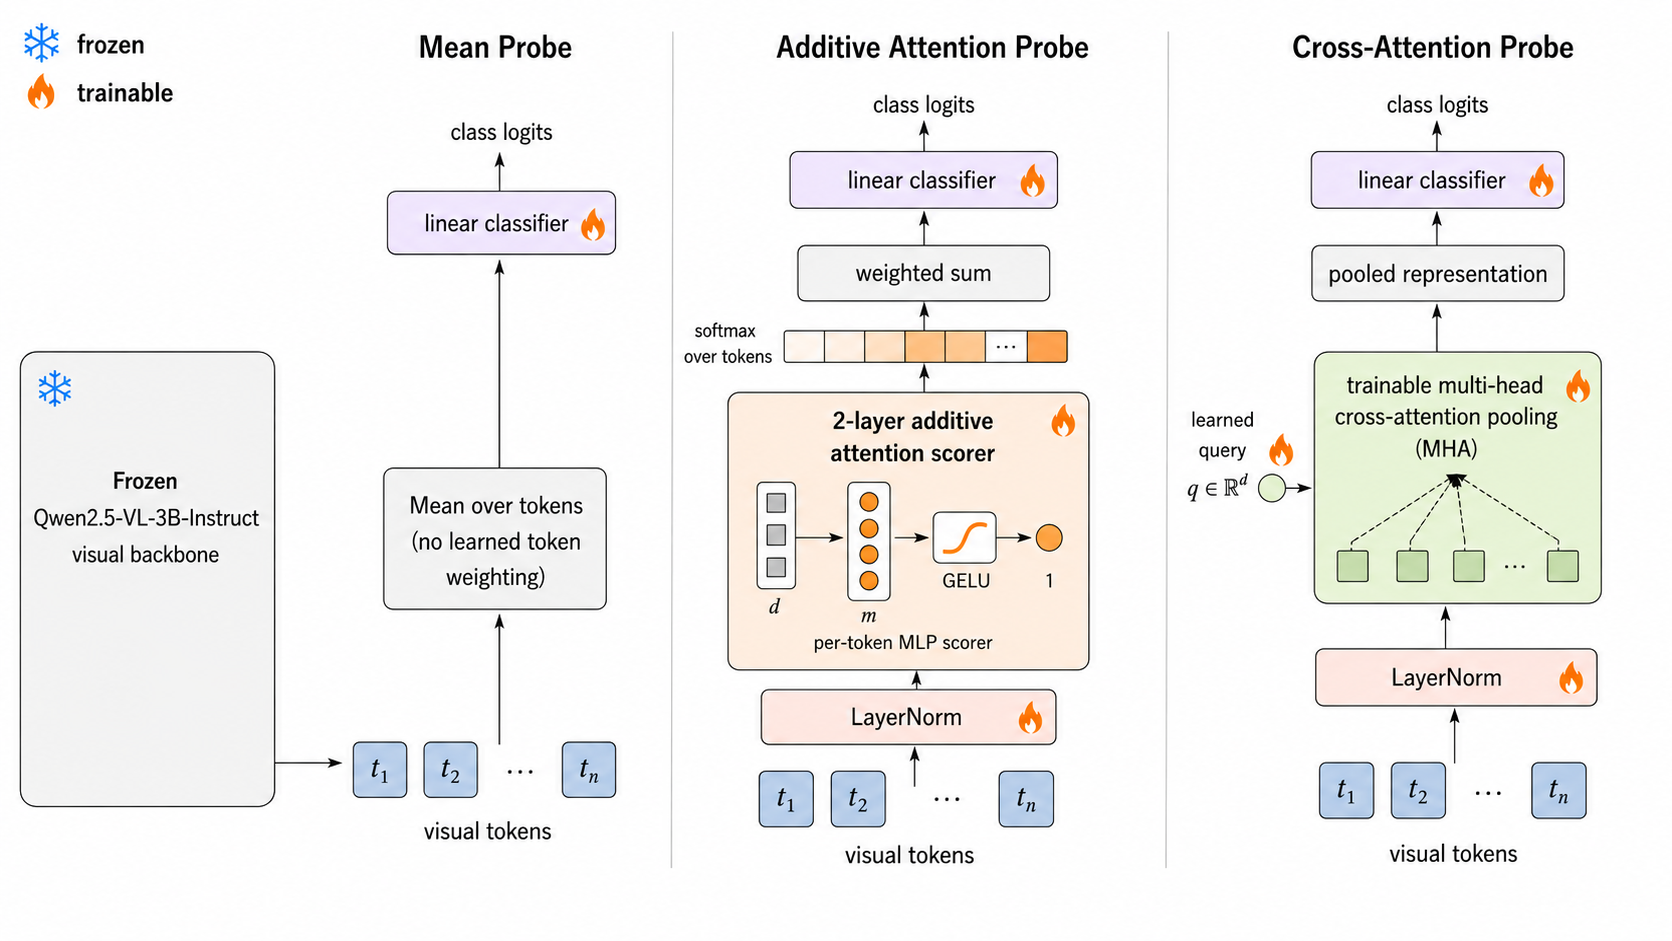
\includegraphics[width=\textwidth]{images/probes.png}
  \caption{Probe-head architectures tested.}
  \label{fig:probe-heads}
\end{figure}

All probe classifiers use zero dropout at the classification head.
Probe training uses AdamW for 10 epochs with batch size 16, learning rate $3\times10^{-4}$, weight decay 0.01, warmup ratio 0.1, cosine learning-rate decay, gradient clipping at norm 1.0 and seed 42 for reproducibility.
The checkpoint used for saliency computation is the best one on the validation set.

\paragraph{Grad-CAM token weights.}
For each image, the frozen Qwen visual backbone produces a token sequence $\{t_i\}_{i=1}^N$.
A trained probe reads these tokens and predicts logits.
We take the class predicted by the probe and ask which visual tokens most supported that logit.
To answer this, Grad-CAM backpropagates the selected logit through the probe head and classifier to the visual tokens.

Because the visual backbone is fixed, differences among the resulting Grad-CAM maps arise from the trained pooling and classification paths from $T$ to the selected logit.

For each probe we backpropagate the target logit through the probe and compute a token-level Grad-CAM score
\begin{equation}
  c_i = \operatorname{ReLU}\left(\sum_d
  \frac{\partial y_k}{\partial t_{i,d}}\,t_{i,d}\right),
\end{equation}
where $y_k$ is the logit of the probe-predicted class and $d$ indexes the feature dimensions of token $t_i$.
The raw scores are normalized per image and sharpened with a softmax temperature $\tau=0.05$ to obtain the final token weights $A_i$.
If the scores are degenerate or non-finite, the example falls back to uniform token weights.


\subsection{Distillation}

\paragraph{Matching teacher and student tokens.}
The probe and the student initially describe the image at different spatial granularities.
At the resolution used in the experiments, the probe assigns relevance weights on a $28\times28$ Qwen token map, while the ViT-B/16 student produces $14\times14=196$ patch tokens from its $224\times224$ input.
We resize the probe relevance map to $14\times14$ and normalize the resulting 196 weights to sum to one.

The teacher target is Qwen's sequence of 196 image embeddings: these are the visual representations normally provided to the language model when it generates an answer.
The student also produces 196 token embeddings, and a learned linear projection maps each student token to the dimension of the teacher.

We compare three distillation objectives.
The baseline aligns the mean visual embedding of the student and teacher using a mean-squared error loss:
\begin{equation}
  \mathcal{L}_{global} = \left\lVert \frac{1}{N}\sum_{i=1}^{N} s_i - \frac{1}{N}\sum_{i=1}^{N} t_i \right\rVert_2^2.
\end{equation}
where $N$ is the number of aligned visual token locations, $t_i$ is the Qwen teacher embedding at location $i$, $s_i$ is the projected student embedding at the same location, and $A_i$ is the resized and normalized relevance weight assigned to location $i$.
The explanation-guided objective uses the aligned token-level weights $A_i$ to concentrate supervision on salient teacher regions:
\begin{equation}
  \mathcal{L}_{expl} = \sum_{i=1}^{N} A_i \left\lVert s_i - t_i \right\rVert_2^2.
\end{equation}
The combined loss is a weighted sum,
\begin{equation}
  \mathcal{L} = \lambda_g\,\mathcal{L}_{global} + \lambda_e\,\mathcal{L}_{expl},
\end{equation}
where $\lambda_g, \lambda_e \ge 0$ control the balance between global reconstruction and explanation-weighted local matching. 

We evaluate three settings: (1) $\lambda_g=1, \lambda_e=0$ (global MSE baseline); (2) $\lambda_g=0, \lambda_e=1$ (explanation-only local matching); and (3) $\lambda_g=1, \lambda_e=1$ (combined objective).

Teacher features and token weights are precomputed before student training.
For the global MSE baseline, the teacher is the vision part of Qwen2.5-VL-3B.
For explanation-guided variants, the teacher is the validation-best probe checkpoint and token weights are Grad-CAM saliency weights derived from the probe logits.
The student is a ViT-B/16 at 224-pixel resolution, followed by a projection into the teacher feature dimension.

\paragraph{Distillation training details.}
Student training uses AdamW for at most 20 epochs with train batch size 16, precompute batch size 4, learning rate $3\times10^{-4}$, weight decay 0.05, warmup ratio 0.1, cosine learning-rate decay, gradient clipping at norm 1.0 and seed 42 for reproducibility.
Early stopping monitors validation distillation loss with patience 5; reported results use the validation-best student checkpoint.

\subsection{Evaluation Metrics}
\label{sec:metrics}


We report three families of metrics. First, teacher probes are measured by validation accuracy and test accuracy. Second, student distillation is measured on validation and test sets using the loss objectives defined above: global MSE, explanation-weighted MSE, and the combined loss. Third, downstream VLM behavior is measured through generated-answer comparison, using an LLM jury: independent VLM judges see the original image and two anonymized answers (that are, the student and teacher answers), then select the better answer or a tie, without any information about which answer is from the teacher or the student. We report majority preference over the three judges on examples where all judges return valid structured outputs. For the judge panel, we employ the \emph{all-judge agreement} as the fraction of examples where all three judges select the same class, and Fleiss' $\kappa$ estimates agreement to measure inter-judge reliability beyond chance. The judge panel is made up of three local VLMs: Qwen3.5-9B~\citep{qwen2026qwen35}, GLM-4.6V-Flash~\citep{vteam2025glm45v}, and MiniCPM-V-4.5~\citep{yu2025minicpmv45}.
Each LLM is loaded with a context length of 32,768 and temperature 0.0.
The generated teacher and student answers are capped at 128 new tokens before judging.
Both text-only and image-grounded judges are constrained to return a structured JSON.
We report the results considering only the subset of examples where all three judges return a valid structured preference.


\section{Results}
\label{sec:results}

\paragraph{Teacher Probe Results.}

The three teacher probes all reach high Mini-ImageNet accuracy on frozen VLM visual features, supported by the fact that the dataset was part of the original VLM pretraining.
This matters because the probes are saliency sources: a stronger or more complex probe is useful only if its gradients provide better distillation guidance.
Table~\ref{tab:probe-results} shows that the mean probe obtains the highest validation and test accuracy.

\begin{table}[H]
  \centering
  \caption{Teacher-probe results on frozen VLM visual features.}
  \label{tab:probe-results}
  \small
  \begin{tabular}{@{}lrrr@{}}
    \toprule
    Probe type & Best epoch & Val accuracy & Test accuracy  \\
    \midrule
    Mean & 10 & \textbf{95.07} & \textbf{95.00} \\
    Attention & 2 & 94.93 & 94.48 \\
    Cross-attn & 10 & 94.58 & 94.78 \\
    \bottomrule
  \end{tabular}
\end{table}


\paragraph{Generated-Answer Results.}

Table~\ref{tab:primary-results} reports the primary image-grounded preference results on a shared subset of 437 images, retaining an image only when all three judges produced valid preferences for every student variant, from the original 500 pool of images.
The teacher remains preferred for most images in every condition, so the current students should not be viewed as complete replacements for the original visual pathway.
The important comparison is between student variants.
Plain global reconstruction is weak: the baseline receives only 10 student-majority wins.
Every explanation-guided variant improves on this baseline, and the best variant, mean-probe explanation-only distillation, receives 69 student-majority wins.


\begin{table}[t]
  \centering
  \caption{LLM jury results}
  \label{tab:primary-results}
  \scriptsize
  \setlength{\tabcolsep}{2.2pt}
  \begin{tabular}{@{}lrrrrr@{}}
    \toprule
    Variant & Student & Teacher & Not Majority & All Agree &  $\kappa$ \\
    \midrule
    Base MSE & 10 & 427 & 0 & \textbf{0.936} &  0.312 \\
    Mean, loss expl. & \textbf{69} & 367 & 1 & 0.705 &  0.355 \\
    Attn, loss expl. & 56 & 381 & 0 & 0.741 &  0.367 \\
    Cross, loss expl. & 20 & 416 & 1 & 0.856 &  0.337 \\
    Mean, loss MSE+expl. & 58 & 379 & 0 & 0.737 &  0.355 \\
    Attn, loss MSE+expl. & 61 & 376 & 0 & 0.737 &  0.338 \\
    Cross, loss MSE+expl. & 37 & 400 & 0 & 0.817 &  \textbf{0.372} \\
    \bottomrule
  \end{tabular}
\end{table}


\subsection{Qualitative Analysis}
\label{sec:qualitative}

Figure~\ref{fig:qualitative-patterns} illustrates what changes in the generated answers when the student is trained with explanation guidance.
In the first two cases, the guided student preserves visible evidence that the global MSE baseline loses: it describes the texture of the mushroom cap more precisely and recognizes the bowls instead of inventing shoes. The lower two examples also show the limit of this result. For the Triceratops skull, the guided student identifies the main object but misses the person and wider scene context captured by the teacher. In the second skeleton example, explanation guidance prevents the severe baseline failure of claiming that no image is available, a problem observed when the distilled visual embeddings do not lie in the distribution expected by the language model. Taken together, these cases indicate improved visual grounding and robustness.


\begin{figure}[t]
  \centering
  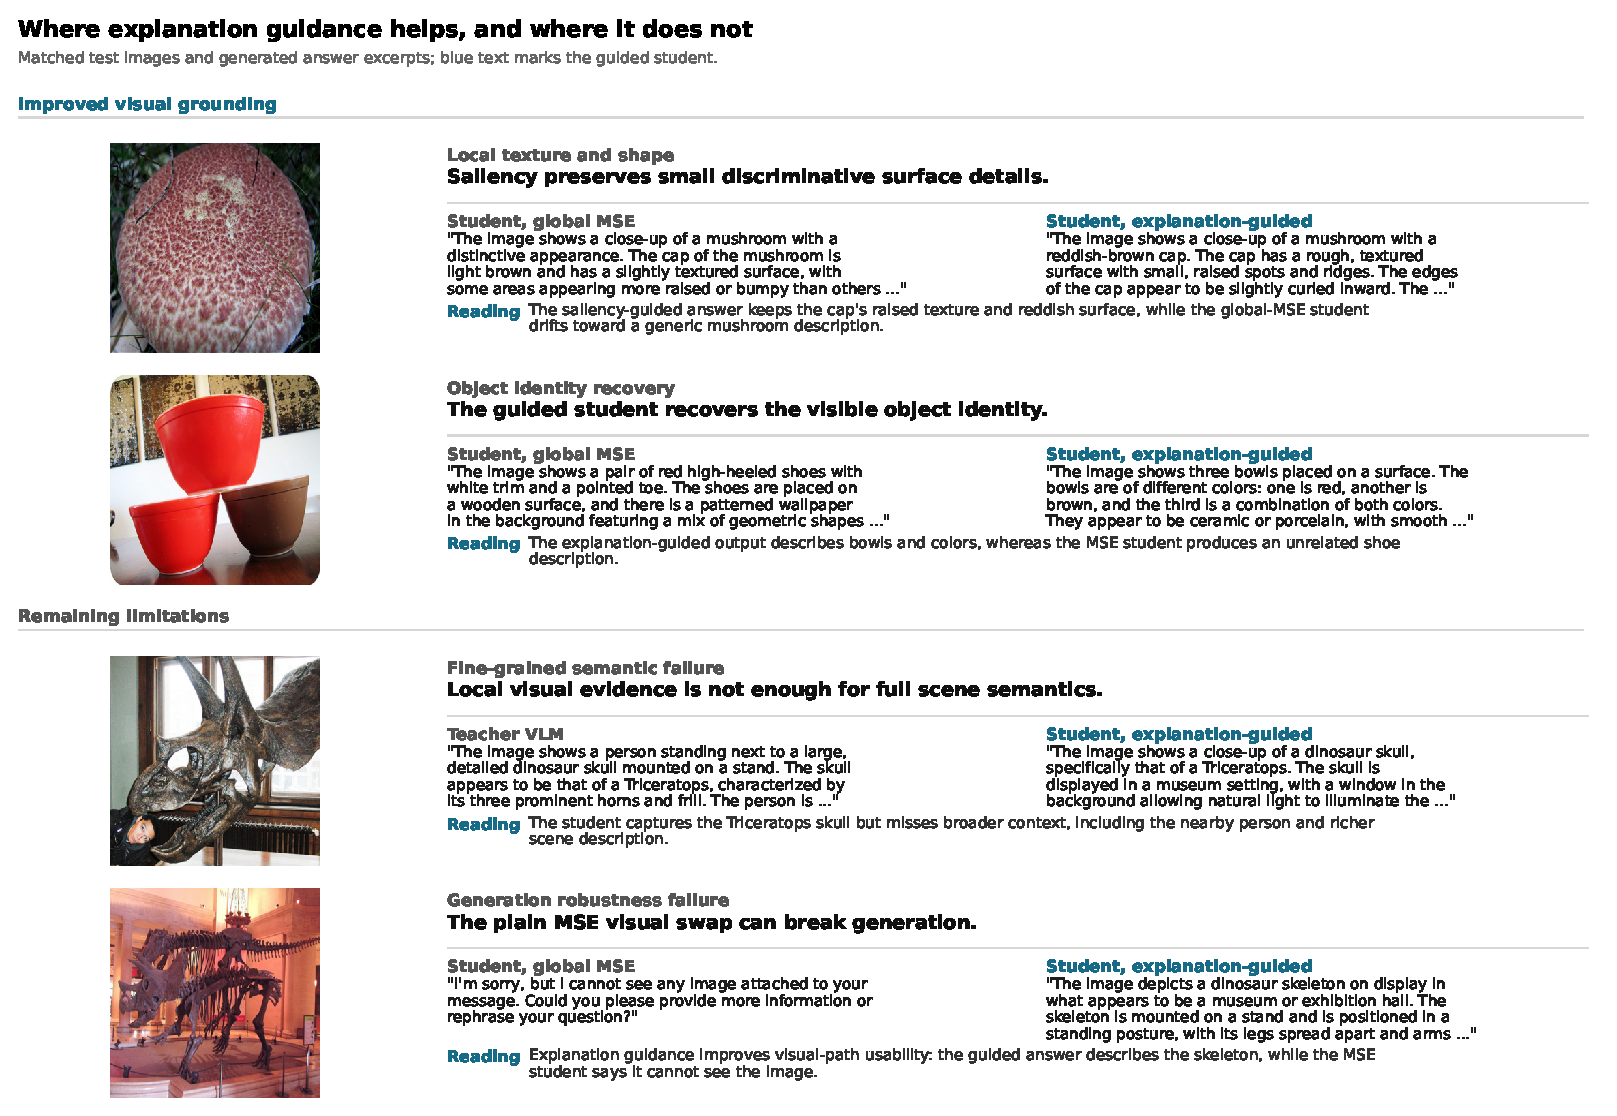
\includegraphics[width=\textwidth]{images/qualitative_patterns_combined}
  \caption{Representative qualitative patterns in generated answers. The upper cases illustrate visual evidence preserved by explanation-guided distillation; the lower cases expose remaining limitations or baseline failure modes.}
  \label{fig:qualitative-patterns}
\end{figure}


\section{Limitations}
\label{sec:limitations}

This study evaluates one teacher VLM, one dataset, and one prompt family.
The conclusions should therefore be read as evidence that explanation-guided distillation is promising, not as a universal result across VLMs.
The judges are VLMs rather than human annotators, so their preferences may contain model-specific biases even under blind answer ordering.
The saliency signal is also mediated by a probe, which may emphasize class-discriminative evidence rather than every detail needed for open-ended generation.
Finally, the current students remain clearly below the teacher in absolute preference, which means the method improves replacement fidelity but does not yet solve faithful visual-module substitution.

\section{Conclusion}
\label{sec:conclusion}

We studied whether explanations can guide knowledge distillation for a VLM visual module.
The student ViT is trained using Grad-CAM-weighted token reconstruction and then plugged into the original VLM so that evaluation happens through generated answers.
Across all tested saliency sources, explanation-guided objectives outperform plain global MSE under image-grounded blind judging.
The strongest result comes from explanation-only supervision, suggesting that explanations can provide a meaningful distillation signal rather than only a secondary regularizer.
Future work should test richer prompts, human preference labels, stronger student adapters, and saliency objectives aligned more directly with the multimodal representation consumed by the language model.


% \section*{Supplementary Material}
% \label{sec:suppl}

% \subsection*{Rationale}
% \label{sec:rationale}

% Having the supplementary compiled together with the main paper means that:

% \begin{itemize}
% \item The supplementary can back-reference sections of the main paper, for example, we can refer to \cref{sec:intro};
% \item The main paper can forward reference sub-sections within the supplementary explicitly (e.g.\ referring to a particular experiment); 
% \item When submitted to arXiv, the supplementary will already included at the end of the paper.
% \end{itemize}

% To split the supplementary pages from the main paper, you can use \href{https://support.apple.com/en-ca/guide/preview/prvw11793/mac\#:\~:text=Delete\%20a\%20page\%20from\%20a,or\%20choose\%20Edit\%20\%3E\%20Delete).}{Preview (on macOS)}, \href{https://www.adobe.com/acrobat/how-to/delete-pages-from-pdf.html\#:\~:text=Choose\%20\%E2\%80\%9CTools\%E2\%80\%9D\%20\%3E\%20\%E2\%80\%9COrganize,or\%20pages\%20from\%20the\%20file.}{Adobe Acrobat} (on all OSs), as well as \href{https://superuser.com/questions/517986/is-it-possible-to-delete-some-pages-of-a-pdf-document}{command line tools}.


\bibliographystyle{unsrtnat}
\bibliography{references}

\end{document}
